%% -*- coding:utf-8 -*- 
\documentclass[14pt,a4paper]{article} 
\usepackage[T1,T2A]{fontenc}
\usepackage[utf8]{inputenc}
\usepackage{minted}
\usepackage{longtable}
\usepackage{hyperref}
\hypersetup{
  pdftex,
  allcolors=blue,
  bookmarksnumbered=true,     
  bookmarksopen=true,         
  bookmarksopenlevel=1,       
  colorlinks=true,            
  pdfstartview=Fit,           
  pdfpagemode=UseOutlines,  
  pdfpagelayout=TwoPageRight,
  pdftitle={Probability paradoxes},
  pdfsubject={Probability},
  pdfauthor={Ivan Murashkо},
  pdfkeywords={probability, paradox}
}
\usepackage{tikz}
\usetikzlibrary{calc,trees,positioning,arrows,fit,shapes,matrix}
\usetikzlibrary{arrows,shapes,positioning}
\usetikzlibrary{decorations.markings}
\title{Probability paradoxes}
\author{Ivan Murashko}
\date{}
\begin{document}

\maketitle
\tableofcontents

\section*{Introduction}
The goal for the article is to demonstrate several paradoxes that are
related to probability theory and how can they can be solved.

\section{Base definitions of probability theory}
We will start with several definitions.

\begin{figure}
  \centering
  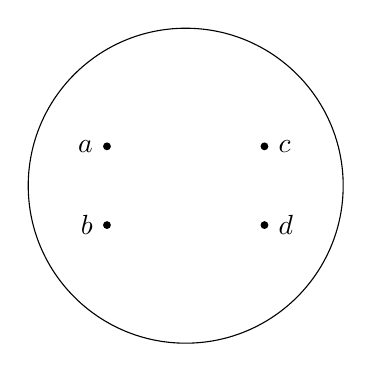
\begin{tikzpicture}[ele/.style={fill=black,circle,minimum
        width=.8pt,inner sep=1pt},every fit/.style={ellipse,draw,inner
        sep=-2pt}]

    % the texts
    \node[ele,label=left:$a$] (a) at (0,2) {};    
    \node[ele,label=left:$b$] (b) at (0,1) {};    
    \node[ele,label=right:$c$] (c) at (2,2) {};
    \node[ele,label=right:$d$] (d) at (2,1) {};
    
    \node[draw,fit= (a) (b) (c) (d),minimum width=4cm, minimum
      height=4cm] {}  ;

  \end{tikzpicture}
  \caption{Probability space. It consists of elementary events: $a$,
    $b$, $c$ and $d$, each
    of them has equal probability $p_{a,b,c,d} = \frac{1}{4}$}
  \label{fig:probabilityspace}
\end{figure}

\begin{figure}
  \centering
  \begin{tikzpicture}[ele/.style={fill=black,circle,minimum
        width=.8pt,inner sep=1pt},every fit/.style={ellipse,draw,inner
        sep=-2pt}]

    % the texts
    \node[ele,color=red] (a) at (0,2) {};    
    \node[ele,top color=green, bottom color=red] (a) at (1,1) {};    
    \node[ele,color=green] (a) at (1,2) {};    
    \node[ele] (b) at (0,1) {};    
    \node[ele] (c) at (2,2) {};
    \node[ele] (d) at (2,1) {};
    
    \node[draw,fit= (a) (b) (c) (d),minimum width=4cm, minimum
      height=4cm] {}  ;

  \end{tikzpicture}
  \caption{Condition probability}
  \label{fig:condprobability}
\end{figure}


TBD \cite{bib:kolmogorov74basic}

\section{Monty Hall problem}
TBD

\section{Waiting time on a bus stop}
TBD

\bibliographystyle{gost780s}  
\bibliography{probability}     


\end{document}
